\documentclass[conference]{IEEEtran}

\usepackage{caption}
\usepackage{subcaption}
\usepackage{grffile}
\usepackage{amsmath}
\usepackage{listings}
\usepackage{enumitem}
\usepackage{color}
\usepackage{mathtools}
\usepackage{algorithm, algpseudocode}

\definecolor{mygreen}{RGB}{28,172,0} % color values Red, Green, Blue
\definecolor{mylilas}{RGB}{170,55,241}

\DeclarePairedDelimiter\abs{\lvert}{\rvert}

\ifCLASSINFOpdf
  \usepackage[pdftex]{graphicx}
\else
\fi

\hyphenation{op-tical net-works semi-conduc-tor}


\begin{document}

\author{\IEEEauthorblockN{David Menager}
\IEEEauthorblockA{School of Electrical Engineering and Computer Science\\
University of Kansas\\
Lawrence, Kansas 66045\\
Email: dhmenager@ku.edu}}

\lstset{language=Matlab,%
    %basicstyle=\color{red},
    breaklines=true,%
    morekeywords={matlab2tikz},
    keywordstyle=\color{blue},%
    morekeywords=[2]{1}, keywordstyle=[2]{\color{black}},
    identifierstyle=\color{black},%
    stringstyle=\color{mylilas},
    commentstyle=\color{mygreen},%
    showstringspaces=false,%without this there will be a symbol in the places where there is a space
    numbers=left,%
    numberstyle={\tiny \color{black}},% size of the numbers
    numbersep=9pt, % this defines how far the numbers are from the text
    emph=[1]{for,end,break},emphstyle=[1]\color{red}, %some words to emphasise
    %emph=[2]{word1,word2}, emphstyle=[2]{style},    
  }
\title{On the Construction of Evolutionary Features for General Object Recognition}
\maketitle

\begin{abstract}
  Object recognition is an important part in computer vision that that allows many computer programs to see the light of day. There are many open problems in this area, and in this paper, we examine a particular approach that uses evolutionary methods for constructing salient features of images. These features are then combined in an ensemble classifier to predict an object class. The performance of this system is reportedly state-of-the-art, and we present our methodology and show that our system fails to meet this expectation due to the time constraints required for the completion of this paper.
\end{abstract}

\IEEEpeerreviewmaketitle

\section{Introduction}
Many theories in artificial intelligence (AI) become reduced to the realm of ``cool ideas'' without computers that can actualize them in the world in which we live. This is not only true for classical AI tasks such as heuristic search, but for other high level tasks such as completing a search and rescue mission, or inferring other people's goals in an environment. High level tasks such as these fundamentally rely on computer vision modules that allow agents to sense the world. In practice, however, researchers tend to avoid this topic by implementing their solutions in simulations. This allows them to develop strong theories that generalize to diverse environments, but often times the research makes assumptions that the vision problem is already solved. Obviously, this is not true.

There is a wealth of research that aims to tackle the different aspects of computer vision. These works address a breadth of topics such ass 3D reconstruction, remote sensing, and augmented reality. Since we are interested in vision modules for physical agents, we will focus this paper on object recognition. Object recognition is the task of assigning an image to a particular object class. In the standard case, each picture images one object, and thus belongs to one object class. In the supervised context, these classes are known a priori and are associated to their corresponding images in a training set. Then the validation of the models are done by using a hold-out set. A procedure like this bares a strong resemblance to the standard machine learning approach, and in fact object recognition, and pattern matching in general, can be seen as a machine learning problem. This relationship between machine learning and object recognition also implies that in order to produce a quality model, a significant amount of work must be done to clean the data that these models consume. Typically, methods for recognizing objects in images are sensitive to:
\begin{description}
\item [Lighting conditions]
  Images of the same object may be subject to different lighting conditions. This difference is potentially enough to mis-classify an object.
\item [Position of the object]
  Many algorithms have better performance if the object to recognize is centered in the image at the foreground. Object recognition becomes significantly more challenging when no constraints are placed on the location of the object.
\item [Orientation of the object]
  Object recognition algorithms can be sensitive to the orientation of the imaged object because these systems analyze the intensity values of pixels, and do not inherently extract semantic information from images without further processing.
\item [Size of the object]
  As the size of the image object varies, the level of detail will also fluctuate, and so this is another issue object recognition systems must address because the number and quality of features in an object can change.
\item [Amount of occlusion of the object]
  Occluded objects are a significant challenge to object recognition systems. Many important features of an object may be missing because they are hidden by another object. 
\item [etc.]
  Various other factors such as the color of an object, or the number of objects to recognize in an image affect the quality of object recognition systems.
\end{description}

All of these give an intuition of the challenging nature of object recognition tasks. In general, it is very difficult to determine which features of an image help to identify the class of an object, given that it may be subject to various levels of noise. Furthermore, the quality of results obtain by these methods are highly dependent on the quality of the datasets being used to train the vision modules. Object recognition is an important research area in computer vision because the success of other, more high-level tasks like extracting relational, or propositional information from 2D images depend on it.

There are many techniques for object recognition \cite{sukanya2016survey}, however in this paper we aim to do this using an ensemble of perceptrons, who have been trained by evolution. This method, proposed by \cite{lillywhite2013feature} performs comparably to deep architectures built for this task, which yield state-of-the art performance. We begin this paper with a review of the genetic algorithm, then we move to explain our experimental setup and compare it with \cite{lillywhite2013feature}. Following this, we provide our results and close with concluding remarks. 
\section{Genetic Algorithm Review}
Genetic algorithms simulate evolution. The idea is to create a program that solves problems by using the well-established principles of Darwinian evolution. In essence, the aim is to create programs that solve problems without needing to be told {\it how} to solve them \cite{koza1992genetic}. Genetic algorithms first begin by initializing a random population. Every individual in a population is represented as a gene vector, where each element in that vector is a feature of that individual. Each individual attempts the problem and is assigned a fitness score based on how well the individual solves that problem. Based on the fitness score, the most fit individuals are selected to pass on their genes to the next generation. Through the processes of sexual recombination (cross over) and mutation, the next generation is created. This process continues for $N$ generations, or until some other stopping criteria is reached.

The cross over procedure is quite simple. In order to generate a new individual from sexual recombination, it suffices to choose a cross over point in each parent. Then, choose the parent whose genes form the beginning of the child, and stitch the end of the second parent's genes to the end of the new child's. After a child has been created in this way, mutations may occur that change the child's specific feature values. More intense mutations may occur by deleting or adding entire elements. From this, it is easily seen that genetic algorithms can span the set of possible solutions because solutions are of non-uniform size and mutations allow the solutions to explore new places in the search space.

Genetic algorithms are attractive particularly because of their broad applicability to optimization problems. As long as a problem can be stated in terms of the aforementioned process, genetic algorithms are good candidates for finding high quality solutions to them. Other than the formalisms inherently embedded in the procedure, and knowledge about the problem do main, no other mathematical constructions are required. For instance, the problem optimal control may be approached with a genetic algorithm. If the programmer is trying to control a UAV and knows what low-level motor actions the UAV can perform, then minimizing the error between the craft's actual state and the desired state becomes a task for evolution. 

In a formal setting, genetic algorithms solve problems by an approach similar to gradient ascent, called {\it hill climbing}. In gradient ascent, the optimal solution is found by going in the direction of the gradient. On a 3-dimensional convex function, going up the gradient will potentially change all three values of the solution vector instantaneously. This contrasts with hill climbing because, for the case of hill climbing, generating the next solution only involves modifying a set of components from the original solution vector. In other words, new solutions are created by copying part of an old solution and adding a set of new pieces that complete the solution. It may not be immediately clear to the reader, but applying cross over with two parent individuals is hill climbing in the context of the genetic algorithm.

\subsection{Why it Works}
Now, we consider why the genetic algorithm works. We do not supply a formal proof, but give a strong intuition. The reason why genetic algorithms work is because in each generation they select the most fit individuals to produce the next. Therefore the average fitness of each successive generation is non-decreasing. DO MORE WORK HERE.
\section{Experimental Comparison}
In this section we take the time to compare our experimental setup with that of \cite{lillywhite2013feature}. We begin by discussing the commonalities and proceed to discuss the differences.
\subsection{Commonalities in approach}
Here we describe, in large part the original paper's implementation and formalisms. In our project, our aim was to remain as faithful to the original theory as possible. We largely embrace the same formalisms, but deviate mostly in the system parameters
\subsubsection{ECO Features and Perceptrons}
Perhaps, the strongest commonality to mention is that our work is a re-implementation of Lillywhite et al. The task is to devise an evolutionary algorithm to construct a set of features that improve a classification algorithm's ability to distinguish object classes. For this reason, the features are called {\it ECO features}, because they are {\bf E}volutionarily {\bf Co}nstructed. An ECO feature, $V$ is simply an ordering of image transformations with their accompanying parameters and is formalized as
\begin{equation}
  \begin{split}
    V_n & = T_n(V_{n-1}, \phi)\\
    V_{n-1} & = T_{n-1}(V_{n-2},\phi_{n-1})\\
    \vdots\\
    V_1 & = T_1(I(x_1,y_1,x_2,y_2), \phi_{1}),
  \end{split}
  \label{eq:eco}
\end{equation}
where $I$ is the original image, $T_i$ is an image transform, and $\phi$ is the set of corresponding parameters to that transform. Figure~\ref{fig:eco-feat} shows Equation~\ref{eq:eco} graphically. After $I$ has been transformed into $V$ by all the transforms ${\bf T}$, it is fed through an associated perceptron. Lillywhite et al. also describe the ability to apply these ECO features to particular subregions of the image. The subregion is defined by $x_1, x_2, y_1,$ and $y_2$, but we chose not to implement the subregions feature because the original authors obtained comparable results with the subregions turned off as well.

Furthermore, Lillywhite et al provide a table to show the set of transformations their algorithm employs. In our implementation we only use a subset of these transforms because we utilized another library. Our specific transformations are shown in Table~\ref{tab:transforms}. 
\begin{figure}[t]
\centering
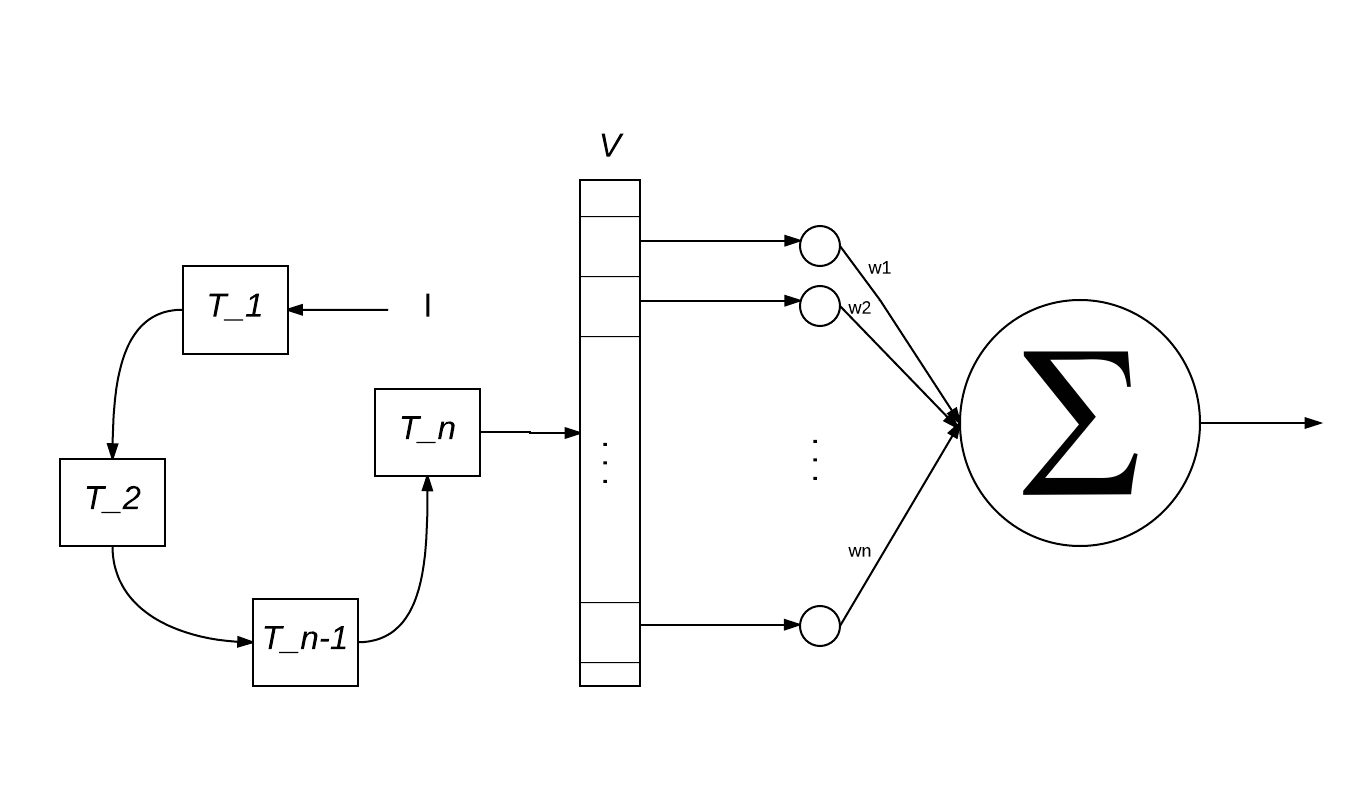
\includegraphics[width=\columnwidth]{eco-feature.png}
\caption{ECO feature block diagram.}
\label{fig:eco-feat}
\end{figure}
\begin{table}[b]
  \centering
  \begin{tabular}{c c c c}
    \hline
    Image Transform & $\abs{\phi}$ & Image Transform & $\abs{\phi}$\\
    \hline
    Gabor & 9 & Rank Order & 1\\
    Gradient & 2 & Sobel & 1\\
    Gaussian & 2 & Erosion & 2\\
    Histogram & 2 & Hough Line & 1\\
    Hough Circle & 3 & Equalize Histogram & 2\\
    Median Blur & 2 & Laplace Edge & 2\\
    Integral Blur & 1 & Dilation & 2\\
    Canny Edge & 4\\
    \hline
  \end{tabular}
  \caption{Image transforms used in project}
  \label{tab:transforms}
\end{table}

Since this is a genetic algorithm, first generation is initialized randomly. Each candidate ECO feature has an associated perceptron that is used to evaluate the quality of the transformed images. Each pixel in the image is multiplied by its corresponding perceptron weights, the result of which is summed. If the sum is greater than a threshold, ``1'' is the output, otherwise the perceptron outputs 0. The equation for the perceptron output, $\alpha$ is described as the following:
\begin{equation}
  \alpha =
  \begin{cases}
    1, & \text{if } W \cdot V + b > 0\\
    0, & \text{otherswise}
    \end{cases},
  \label{eq:perceptron-output}
\end{equation}
where $W$ is the perceptron weight vector. Furthermore, each image has a class associated that can be discretized as, $\beta$ which is ``1'' for the first image class and ``0'' for the second. So, the error, $\delta$ of the perceptron is written as
\begin{equation}
  \delta = \beta - \alpha.
  \label{eq:perceptron-error}
\end{equation}
This means that training the perceptron is characterized by
\begin{equation}
  W[i] = W[i] + \lambda \cdot \delta \cdot V[i],
  \label{eq:perceptron-update}
\end{equation}
where $\lambda$ is the learning rate. This parameter controls the volatility of the network. High learning rates will cause a network to rapidly oscillate between extreme values. This comes as a trade off to small learning rates that move to convergence. Both high and low learning rates have their disadvantages, however. High learning rates may never converge because the weights bounce around the space of network weights. On the other hand, small learning rates may converge to local maxima and never find an optimal solution. So, the best learning rate, must be found experimentally.

Because Equation~\ref{eq:perceptron-output} through Equation~\ref{eq:perceptron-update} define the fundamental procedures that operate on perceptrons, a fitness function can be defined. Lillywhite et al. specify theirs as

\begin{equation}
  s = \frac{t_p \cdot 500}{f_n + t_p} + \frac{t_n \cdot 500}{p \cdot f_p+ t_n},
  \label{eq:fitness-lilly}
\end{equation}
because it is unaffected by unbalanced classes, and it includes an extra penalty for false positives. In this equation, $t_p, t_n, f_p,$ and $f_n$ stand for true positives, true negative,s false positives, and false negatives respectfully.

\subsubsection{Genetic Algorithm Structure}
Although we discussed the basic genetic algorithm in the previous section, we have yet to define its specific implementation. Lillywhite et al.'s algorithm for evolving features is written in Algorithm~\ref{alg:genetic}.
\begin{algorithm}[t]
  \caption{Genetic Algorithm Outline}
  \label{alg:genetic}
  \begin{algorithmic}
    \For{Size of population}
    \State Randomly create creatures
    \EndFor
    \For{Number of generations}
    \For{Every Creature}
    \For{Every Training Image}
    \State Process the image with feature transformations
    \State Train creature's perceptron
    \EndFor
    \For{Every holding image}
    \State Process the image with feature transformations
    \EndFor
    \State Calculate fitness score
    \State Save creature if sufficiently fit
    \EndFor
    \State Create the next generation
    \EndFor
  \end{algorithmic}
\end{algorithm}

\begin{algorithm}[t]
  \caption{Train AdaBoost}
  \label{alg:ada}
  \begin{algorithmic}
    \State Set of training images M
    \For{Every training image, m}
    \State Initialize $\delta_m[m]=1/|M|$
    \EndFor
    \For{$x=0 \text{ to } X$}
    \For{Every perceptron, $w$}
    \For{Every training image, $m$}
    \If{Wrongly classified}
    \State $\delta_w+=\delta_M[m]$
    \EndIf
    \EndFor
    \EndFor
    \State Select perceptron with minimum Error
    \If{$\delta_\omega[\Omega]>=50\%$}
    \State BREAK
    \EndIf
    \State Calculate perceptron coefficient using
    \State$\rho=\frac{1}{2} \cdot ln\frac{1-\delta_w}{\delta_w}$
    \For{Every training image, $m$}
    \State
    $c =
    \begin{cases}
      1, & \text{if classified correctly}\\
      -1, & \text{otherswise}
    \end{cases}$
    \State $\delta_M[m]=\frac{\delta_M[m]*e^{-\rho \cdot c}}{\text{Normalization factor}}$
    \EndFor
    \EndFor
  \end{algorithmic}
\end{algorithm}

Note, that in Algorithm~\ref{alg:genetic} Lillywhite et al. do not specify how they split their data into training and testing, and more importantly, they do not explain how they process images through the perceptron. Each image has a different size, so in our implementation we fix the number of perceptrons to $\text{max image size } \times \text{max image size}$. Also, observe that once sufficiently fit features are found, the are saved in the list of true ECO features. The list is passed on to create the AdaBoost classifier. This procedure is described by Algorithm~\ref{alg:ada}.

Figure~\ref{fig:ada} shows a block diagram of the AdaBoost classifier. For each classifier, the input image is transformed by the corresponding ECO features. The output of this is multiplied by a perceptron coefficient which determines the amount one perceptron affects the outcome. Then the classification rule is a test to verify that the sum of the perceptron outputs times their coefficients is greater than some threshold $\tau$. 

Our project is a re-implementation of \cite{lillywhite2013feature} that aimed to remain faithful to as many of the theoretical commitments made by the original authors. For the most part we succeeded in achieving this goal, however, external factors such as the time constraint placed on the completion of this project forced us to scale down a few minor aspects of the code. We describe these in the following subsection.
\begin{figure}[t]
  \vskip -.2in
  \centering
  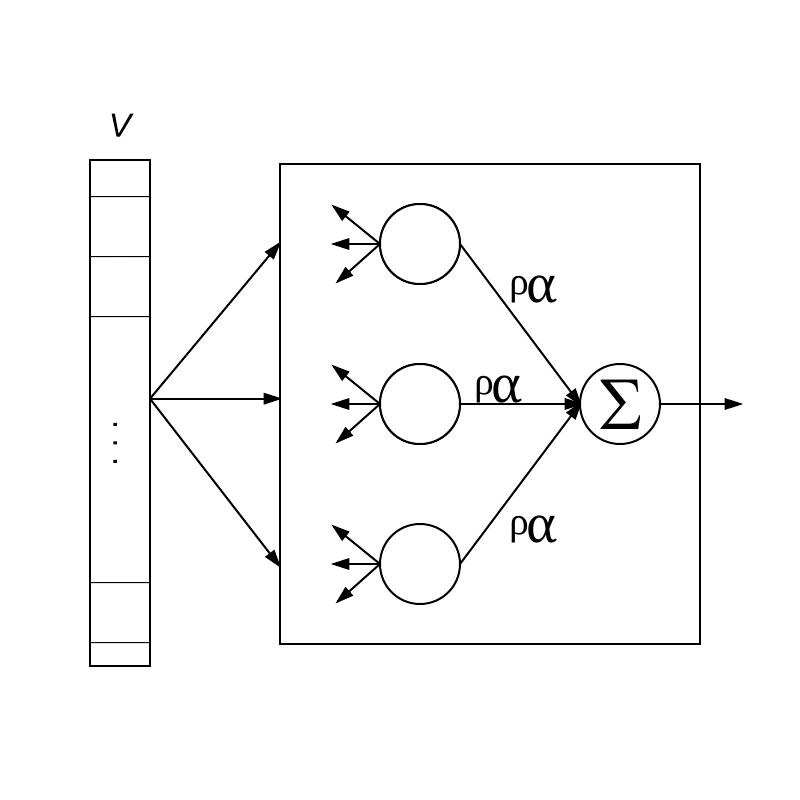
\includegraphics[width=\columnwidth]{ada.png}
  \vskip -.5in
  \caption{AdaBoost feature block diagram.}
  \label{fig:ada}
\end{figure}
\subsection{Differences}
We begin with a discussion on the difference in parameter settings. Lillywhite et al.'s results are generated by an initial population of 1000 individuals who evolve over 100 generations. An algorithmically complex code such as this with the same parameter settings would take the majority of a month to complete on our machines. So, the first modification was to create a population of five individuals who evolve over five generations. The reader might correctly suspect that this is much too short a time to reach convergence. We do not expect our experiment to converge. Rather, we aim to demonstrate the process required to run this genetic algorithm, and we aim to provide preliminary evidence that the evolutionary process is working.

Secondly, Lillywhite et al. state that they only required the initial generation to be no more than eight features long. They also report that the genetic algorithm naturally preferred features with fewer transforms. We are skeptical of this partially because the fitness function does not penalize an individual on the size of it features. We chose to be more restrictive, and specify that all individuals may have at maximum five feature transformations. This specification was a way to artificially append a constraint to the fitness function.

Thirdly, the original paper lacks details with respect to creating generations. The paper does not describe the order in which parents are recombined, does not discuss the number of children two individuals can generate, and the paper is silent about what types of mutations are allowed. In our case, we decided to allow mutations to the transformations and the transformation parameters. We do not add or delete transformations.

Finally, because of the small number of individuals and generations we have a learning rate of 1, mutation probability of .35, add no bias term in Equation~\ref{eq:perceptron-output}, and we include no penalty in our fitness function. The reason why we disagree with the fitness function described in Equation~\ref{eq:fitness-lilly} is because it has poor worst-case performance. We identify two worst-case scenarios:
\begin{enumerate}
\item The perceptron output seems random
\item The perceptron output is constant
\end{enumerate}

In the first case, the fitness function performs reasonably well and penalizes the perceptron for its deviations. The second case contains two subcases, one for each value. If the perceptron output is 1, then Equation~\ref{eq:fitness-lilly} becomes

\begin{equation}
  \begin{split}
    s & = \frac{t_p \cdot 500}{f_n + t_p} + \frac{t_n \cdot 500}{p \cdot f_p+ t_n}\\
    & = \frac{t_p \cdot 500}{0 + t_p} + \frac{0 \cdot 500}{p \cdot f_p + 0}\\
    & = 500(1)
  \end{split}.
  \label{eq:fitness-lilly-decompose}
\end{equation}
For the second subcase, we obtain

\begin{equation}
  \begin{split}
    s & = \frac{t_p \cdot 500}{f_n + t_p} + \frac{t_n \cdot 500}{p \cdot f_p+ t_n}\\
    & = \frac{0 \cdot 500}{f_n + 0} + \frac{t_n \cdot 500}{p \cdot 0 + t_n}\\
    & = 500(1)
  \end{split},
  \label{eq:fitness-lilly-decompose2}
\end{equation}
So, in both cases, if the perceptron does not try to distinguish any classes, it receives a fitness score of 500. On the other hand, a perceptron that attempts to distinguish the two classes will be penalized more because the denominator will include terms for Type I and Type II errors. Furthermore, false positives are penalized heavily. Since the initial generation is created randomly, the features that pass on their traits will be the ones that have no ability to distinguish classes, and the average fitness of the generations will remain at 500. We have empirically seen that ECO features with this trait contain more than 6 transforms.

Our new fitness function shown in Equation~\ref{eq:fitness-menager} avoids this issue in a three-fold manner. First, we include $L_2$ regularization on the length of the feature. Second, our fitness function accounts for the accuracy, precision, and recall of the perceptron, and third, provides a weighting mechanism to prefer accuracy over precision and recall, (and vise versa). This formulation
\begin{equation}
  \begin{split}
    s & = \alpha(\frac{t_p + t_n}{t_p + t_n + f_p + f_n}) +\\
    &(1 - \alpha)(\frac{t_p}{t_p + f_p} + \frac{t_p}{t_p + f_n}) + \lambda \sum_{\bf T} |T_i|
    \end{split}
  \label{eq:fitness-menager}
\end{equation}
penalizes errors in classification, but also heavily penalizes indistinguishability by applying some weightage on the accuracy, precision and recall. In our work, we set $\alpha$ to .4, and the regularization parameter, $\lambda$ is set to 1.

After using this fitness function, we realized that the length of the ECO features were still quite long, so this motivated us to impose the strict 5-feature limit, as mentioned earlier. As future work, we would like to experiment with other regularizers, like using the $L_1$ norm. The downside to this is that this fitness function is sensitive to class imbalance, unlike the one used by Lillywhite et al. 

\section{Results}
In this section we present our results. The results are complete, and a thorough analysis is included, but due to the time constraints and the time complexity of the algorithm, the number of iterations were severely reduced. Lillywhite et al. evolved 100 individuals over 1000 generations. Our results are generated by evolving five individuals over five generations. The reader should not expect spectacular results at this point.

The experiment was completed using images of the American flag, and random backpacks from the Caltech 256 dataset \cite{griffin2007caltech}. Figure~\ref{fig:images} shows a sampling of these.
\begin{figure*}[t]
  \centering
  \begin{subfigure}{.2\textwidth}
    \centering
    \includegraphics[width=\linewidth]{/home/david/Code/courses/eecs_741/256_ObjectCategories/002.american-flag/002_0001.jpg}
  \end{subfigure}
  \begin{subfigure}{.2\textwidth}
    \centering
    \includegraphics[width=\linewidth]{/home/david/Code/courses/eecs_741/256_ObjectCategories/002.american-flag/002_0002.jpg}
  \end{subfigure}
  \begin{subfigure}{.2\textwidth}
    \centering
    \includegraphics[width=\linewidth]{/home/david/Code/courses/eecs_741/256_ObjectCategories/002.american-flag/002_0003.jpg}
  \end{subfigure}
  \begin{subfigure}{.2\textwidth}
    \centering
    \includegraphics[width=\linewidth]{/home/david/Code/courses/eecs_741/256_ObjectCategories/002.american-flag/002_0004.jpg}
  \end{subfigure}
  \begin{subfigure}{.2\textwidth}
    \centering
    \includegraphics[width=\linewidth]{/home/david/Code/courses/eecs_741/256_ObjectCategories/003.backpack/003_0001.jpg}
  \end{subfigure}
  \begin{subfigure}{.2\textwidth}
    \centering
    \includegraphics[width=\linewidth]{/home/david/Code/courses/eecs_741/256_ObjectCategories/003.backpack/003_0002.jpg}
  \end{subfigure}
  \begin{subfigure}{.2\textwidth}
    \centering
    \includegraphics[width=\linewidth]{/home/david/Code/courses/eecs_741/256_ObjectCategories/003.backpack/003_0003.jpg}
  \end{subfigure}
  \begin{subfigure}{.2\textwidth}
    \centering
    \includegraphics[width=\linewidth]{/home/david/Code/courses/eecs_741/256_ObjectCategories/003.backpack/003_0004.jpg}
  \end{subfigure}
  \caption{Input images}
  \label{fig:images}
\end{figure*}

We have two main results, one for the ECO feature construction step, and the other is the AdaBoost classifier metrics. We omit a dedicated Discussion section and embed it herein.
\subsection{ECO Features}
These results are positive and negative. The good news is that the genetic algorithm works as intended. Figure~\ref{fig:fitness} shows the average fitness of the population increase from generation to generation. The problem is that at some point it hits a ceiling. Recall that when its time to produce the next generation, the most fit individuals are selected from the current generation. In this case ``most fit'' means a fitness score above the mean. Results like these imply a number of things:
\begin{description}
\item[Insufficient transforms]
  Our transformations list was a subset of the original authors. It could be that the transformations not present in our experiment bound the fitness at the observed point. Most of the transformations in our list were blurs, edge detection, and filters for detecting geometric shapes. The original authors had these and others like the Fourier transform.
\item[Poor fitness measure]
  It is known that the author's original fitness function is sub optimal because of its bias to rank individuals with no distinguishing ability higher than those that try and make errors. Our novel fitness function arose from realizing the relationship between an individual's ability to distinguish classes and the length of its features. So we decided to penalize lengthy features more. We have not carried out all the necessary analysis to conclude our method is superior to Lillywhite et al's. Because of this, we do not know if our fitness function has biases of its own, nor do we know how to mitigate them, if they exist. 
\item[Poor population size]
  An initial population of five is certainly not sufficient to cover the space of all possible features. This initial size was a severe limiting factor in our performance since, there was only a small pool of candidates to evolve
\item[Poor mutations]
  Moreover, it may have been that our mutations were not occurring frequently enough and/or they were not good enough to discover new, useful features on the surface of the ECO feature space.
\item[Small number of generations]
  Another factor related to this is the number of generations. In our case, the results could only be showing a local maximum. At some time in the future, the fitness may have increased. With five samples, it is hard to draw conclusions about the future performance of the system.
\end{description}
\begin{figure}[t]
\centering
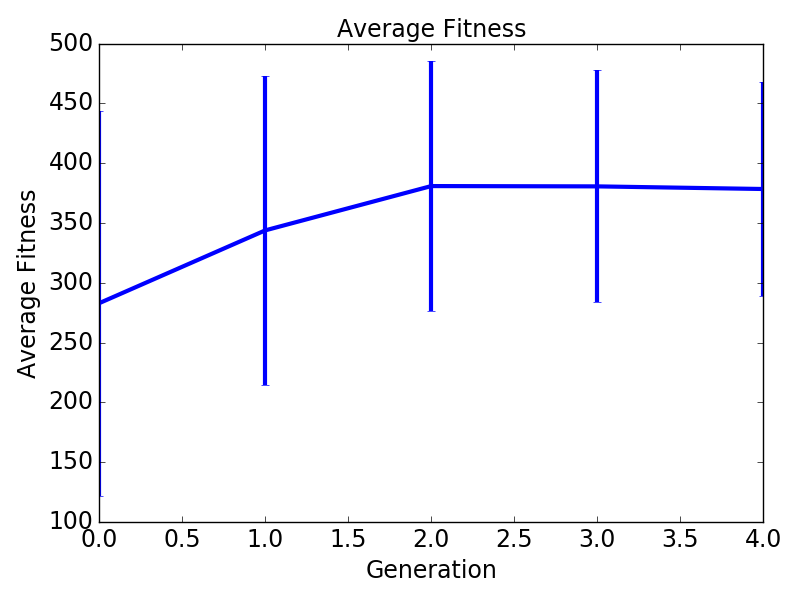
\includegraphics[width=\columnwidth]{average-fitness.png}
\caption{Average fitness of the ECO features through five generations.}
\label{fig:fitness}
\end{figure}
\begin{figure}[t]
\centering
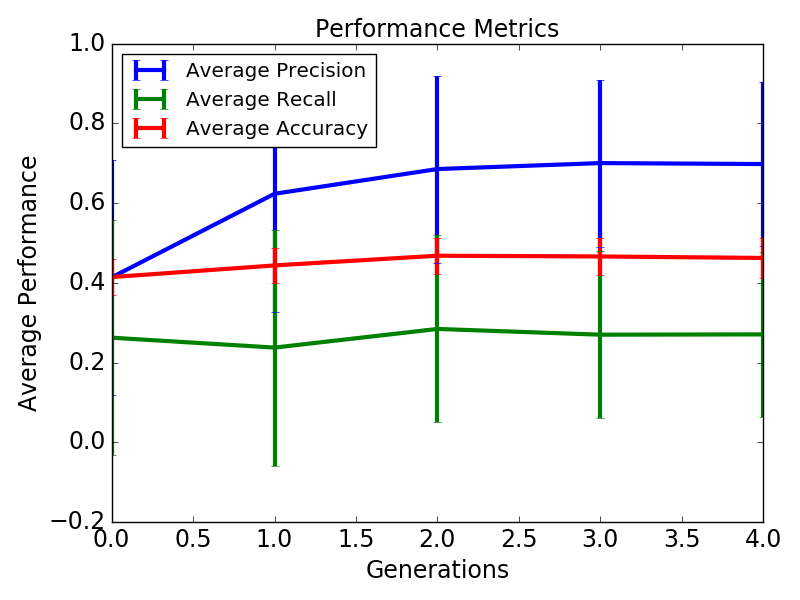
\includegraphics[width=\columnwidth]{average-performance.png}
\caption{Average performance metrics of the ECO features through five generations.}
\label{fig:metrics}
\end{figure}
In our case, we potentially suffer from all four. This is such a complex conundrum that, at this point we are not certain the degree to which these factors affect our result in Figure~\ref{fig:fitness}. Lillywhite et al. report state-of-the-art performance with this technique, so even if they have a bad fitness function, it may be the case that their mutations, cross over procedure, population size, and number of generations were sufficiently good to overcome this. This seems like a reasonable conjecture because Figure~\ref{fig:fitness} shows a pretty high standard deviation. An approximately optimal selection criteria would be able to take advantage of this to produce better quality generations. In our case, we see that the standard deviation is decreasing slightly each generation, signaling the end of genetic diversity in the population.

Furthermore, Figure~\ref{fig:metrics} shows some standard performance metrics of the ECO features from generation to generation. This figure also brings good and bad news. The good news is that the fitness function forces the average precision to increase. On the other hand the recall is low and the average accuracy is more or less constant over the generations. Once again, the performance reaches another ceiling.

As a quick review, precision is the percent of predicted classes that match the true image class. In other words a classifier may make errors, but is precise if whenever it classifies something as belonging to class 'A', that object actually belongs to image class 'A'. Recall is the cousin of this idea, and measures what percent of a particular image class, the classifier captures. For example, a classifier that always predicts one image class has high recall because its predictions cover the entire space of that image class. On average, observe that the ECO feature precision hovers around 65\% in the later generations, and the recall is absolutely underwhelming in all generations. This yields, on average, a classifier with low accuracy, as we see in Figure~\ref{fig:metrics}.
\subsection{AdaBoost}
Because of the poor quality of ECO features, the performance of the AdaBoost classifier will also be poor. Its confusion matrix is shown in the table below. At first glance it is surprising that the classifier only predicts image class 0, which is the American flag in this case. After further inspection, it becomes overwhelmingly clear that this performance is directly caused by the poor quality of ECO features.

\setlength\unitlength{1.5cm}
\begin{center}
  \vskip .3in
  \begin{picture}(3,3)
    \multiput(0.1,0.1)(0,1){3}{\line(1,0){2}}
    \multiput(0.1,0.1)(1,0){3}{\line(0,1){2}}
    \put(0.5,0.5){47}
    \put(1.5,0.5){27}
    
    \put(0.5,1.5){0}
    \put(1.5,1.5){0}
    
    \put(-0.5,1.5){\rotatebox{90}{Flag}}
    \put(-0.5,0.1){\rotatebox{90}{Backpack}}
    
    \put(0.5,2.5){Flag}
    \put(1.1,2.5){Backpack}
    
    \put (-1.2,0.5){\rotatebox{90}{Predicted}}
    \put(0.5,3.2){Actual}
  \end{picture}
\end{center}
From Algorithm~\ref{alg:ada}, recall there is a threshold on the perceptron error. If the minimum perceptron error is greater than the 50\%, in this case, then AdaBoost does not attempt to learn the perceptron coefficients necessary for ensemble classification. Each perceptron coefficient $\rho_i$ is initialized to zero, so when the classification rule is applied, the response is zero. This is the reason why AdaBoost is performing poorly. 

\section{Future Work}
For future work, we plan to reformulate our fitness function and determine its best and worst-case performance. We also plan on running the algorithm with more individuals over more generations. Thirdly, we plan on making a more robust mutation procedure to avoid local optima. Also, incorporating more image transformations would be beneficial. Lastly, we will expand the project by adding more image classes. We will re run the experiments and perform 10-Fold cross validation rather than the holding set approach we used. This will permit us to have a better estimate of the true model performance.
\section{Conclusion}
In this paper we presented our re-implementation of \cite{lillywhite2013feature}. We reviewed the genetic algorithm. After that we compared and contrasted the two implementations, discovered the weaknesses in the original fitness function, then proposed our novel fitness measure. We presented our results and found that they did not quantitatively corroborate the original work. This is partly because the project was subject to time constraints and could not be run for the amount of time Lillywhite et al. reported. The obtained results also suggest that the cross over and mutation procedures are insufficiently robust, and that the population size coupled with the number of generations was too small. We provide the full code in the appendix.
\section{Appendix}
\bibliographystyle{IEEEtran}
\bibliography{IEEEabrv,menager}
\end{document}


